\documentclass{beamer}

\usepackage[skins,theorems]{tcolorbox}
\usepackage{amsmath}
\usepackage{xcolor}
\usepackage{tikz}
\usepackage{pgfplots}
\usepackage{pgfplotstable}

% \usepackage[style=authoryear,backend=biber]{biblatex}
% \addbibresource{bibliography.bib}

\setbeameroption{show notes}

\title[Survival analysis]{An introduction to survival analysis}
\author{Georg W\"olflein}
\institute[www.st-andrews.ac.uk]{School of Computer Science, University of St Andrews}
\titlegraphic{
\includegraphics[width=0.1\paperwidth]{./figs/crest.pdf}}


\usetheme{Berlin}

\usetikzlibrary{decorations.pathreplacing,calc,positioning}
\pgfplotsset{compat=1.18}

\newcommand{\tikzmark}[1]{\tikz[overlay,remember picture] \node (#1) {};}

\newcommand{\prob}[1]{\ensuremath{\Pr{\left(#1\right)}}}

%%%%%%%%%%%%%%%%%%%%%%%%%%%%%%%%%%%%
%%%       Highlighter code       %%%
%%%%%%%%%%%%%%%%%%%%%%%%%%%%%%%%%%%%
\makeatletter


\tikzset{%
  remember picture with id/.style={%
    remember picture,
    overlay,
    save picture id=#1,
  },
  save picture id/.code={%
    \edef\pgf@temp{#1}%
    \immediate\write\pgfutil@auxout{%
      \noexpand\savepointas{\pgf@temp}{\pgfpictureid}}%
  }
}

\def\savepointas#1#2{%
  \expandafter\gdef\csname save@pt@#1\endcsname{#2}%
}

\tikzdeclarecoordinatesystem{pic}{%
  \@ifundefined{save@pt@#1}{%
    \pgfpointorigin
  }{%
  \pgfsys@getposition{\csname save@pt@#1\endcsname}\save@orig@pic%
  \pgfsys@getposition{\pgfpictureid}\save@this@pic%
  \pgf@process{\pgfpointorigin\save@this@pic}%
  \pgf@xa=\pgf@x
  \pgf@ya=\pgf@y
  \pgf@process{\pgfpointorigin\save@orig@pic}%
  \advance\pgf@x by -\pgf@xa
  \advance\pgf@y by -\pgf@ya
  }%
}

\newcounter{highlight}
\newcommand{\hlstart}{\tikz[remember picture with id=hlstart\the\value{highlight},baseline=-0.7ex];\hl@start}
\newcommand{\hlend}{\tikz[remember picture with id=hlend\the\value{highlight},baseline=-0.7ex];\hl@end\stepcounter{highlight}}
\newcommand{\fdstart}{\tikz[remember picture with id=hlstart\the\value{highlight},baseline=-0.7ex];\fd@start}
\newcommand{\fdend}{\tikz[remember picture with id=hlend\the\value{highlight},baseline=-0.7ex];\fd@end\stepcounter{highlight}}
\newcommand{\vlstart}{\tikz[remember picture with id=hlstart\the\value{highlight},baseline=-1em];\vl@start}
\newcommand{\vlend}{\tikz[remember picture with id=hlend\the\value{highlight},baseline=0.3ex];\vl@end\stepcounter{highlight}}

\newcommand{\hl@start}[1][]{%
  \hl@draw{highlighter}{#1}{\the\value{highlight}}}

\newcommand{\hl@end}{}

\newcommand{\fd@start}[1][]{%
  \def\fd@args{#1}}

\newcommand{\fd@end}{\def\@tempa{\hl@draw{fader}}\expandafter\@tempa\expandafter{\fd@args}{\the\value{highlight}}\def\fd@args{}}

\newcommand{\vl@start}[1][]{%
  \vl@draw{highlighter}{#1}{\the\value{highlight}}}

\newcommand{\vl@end}{}


\def\hl@sets{%
  \edef\hl@sx{\the\pgf@x}%
  \edef\hl@sy{\the\pgf@y}%
}
\def\hl@sete{%
  \edef\hl@ex{\the\pgf@x}%
  \edef\hl@ey{\the\pgf@y}%
}

\@ifclassloaded{beamer}{

  \def\page@node{
    \path (current page.south east)
        ++(-\beamer@rightmargin,\footheight)
    node[
      minimum width=\textwidth,
      minimum height=\textheight,
      anchor=south east
    ] (page) {};
  }

}{

  \def\page@node{
    \path (current page.north west)
    ++(\hoffset + 1in + \oddsidemargin + \leftskip,\voffset + 1in + \topmargin + \headheight + \headsep)
    node[
      minimum width=\textwidth - \leftskip - \rightskip,
      minimum height=\textheight,
      anchor=north west
    ] (page) {};
  }

}

\newcommand{\hl@draw}[3]{%
  \begin{tikzpicture}[remember picture,overlay]%
  \page@node
  \tikzset{#2,highlight=#1,every path/.append style={highlight=#1}}%
  \pgfmathsetlengthmacro{\hl@width}{\the\pgflinewidth - 1pt}%
  \coordinate (hlstart) at (pic cs:hlstart#3);
  \coordinate (hlend) at (pic cs:hlend#3);
  \tikz@scan@one@point\hl@sets(pic cs:hlstart#3)
  \tikz@scan@one@point\hl@sete(pic cs:hlend#3)
  \ifdim\hl@sy=\hl@ey\relax
  \draw (hlstart) -- (hlend);
  \else
  \draw (hlstart) -- (hlstart -| page.east);
  \pgfmathsetlengthmacro{\hl@sy}{\hl@sy -\hl@width}%
  \pgfmathsetlengthmacro{\hl@ey}{\hl@ey +\hl@width}%
  \loop\ifdim\hl@sy>\hl@ey\relax
  \draw (0,\hl@sy -| page.west) -- (0,\hl@sy -| page.east);
  \pgfmathsetlengthmacro{\hl@sy}{\hl@sy -\hl@width}%
  \repeat
  \draw (hlend -| page.west) -- (hlend);
  \fi
  \end{tikzpicture}%
}

\newcommand{\vl@draw}[3]{%
  \begin{tikzpicture}[remember picture,overlay]%
  \page@node
  \tikzset{#2,highlight=#1,every path/.append style={highlight=#1}}%
  \pgfmathsetlengthmacro{\hl@width}{\the\pgflinewidth - 1pt}%
  \coordinate (hlstart) at (pic cs:hlstart#3);
  \coordinate (hlend) at (pic cs:hlend#3);
  \tikz@scan@one@point\hl@sets(pic cs:hlstart#3)
  \tikz@scan@one@point\hl@sete(pic cs:hlend#3)
  \ifdim\hl@sx=\hl@ex\relax
  \draw (hlstart) -- (hlend);
  \else
  \draw (hlstart) -- (hlstart |- page.south);
  \pgfmathsetlengthmacro{\hl@sx}{\hl@sx -\hl@width}%
  \pgfmathsetlengthmacro{\hl@ex}{\hl@ex +\hl@width}%
  \loop\ifdim\hl@sx>\hl@ex\relax
  \draw (\hl@sx,0 |- page.north) -- (\hl@sx,0 |- page.south);
  \pgfmathsetlengthmacro{\hl@sx}{\hl@sx -\hl@width}%
  \repeat
  \draw (hlend |- page.north) -- (hlend);
  \fi
  \end{tikzpicture}%
}

\tikzset{%
  highlight/.default=highlighter,
  highlight/.style={
    color=\pgfkeysvalueof{/tikz/#1 colour},
    line width=\pgfkeysvalueof{/tikz/#1 width},
    line cap=\pgfkeysvalueof{/tikz/#1 cap},
    opacity=\pgfkeysvalueof{/tikz/#1 opacity},
  },
  highlighter colour/.initial=yellow,
  highlighter width/.initial=14pt,% <-- Tweak (was 12pt)
  highlighter cap/.initial=butt,
  highlighter opacity/.initial=1,
  fader colour/.initial=gray,
  fader width/.initial=12pt,
  fader cap/.initial=butt,
  fader opacity/.initial=.5,
}



\@ifclassloaded{beamer}{

%% Beamer variants

\setbeamercolor{highlighted text}{bg=yellow}
\setbeamercolor{faded text}{fg=gray}

\newcommand<>{\highlight}[2][]{%
  \only#3{\hlstart[#1]}#2\only#3{\hlend}}

\newcommand<>{\fade}[2][]{%
  \only#3{\fdstart[#1]}#2\only#3{\fdend}}

\newcommand<>{\vhighlight}[2][]{%
  \only#3{\vlstart[#1]}#2\only#3{\vlend}}

}{

\newcommand{\highlight}[2][]{%
\hlstart[#1]#2\hlend}

\newcommand{\fade}[2][]{%
\fdstart[#1]#2\fdend}

\newcommand{\vhighlight}[2][]{%
\vlstart[#1]#2\vlend}}

\def\hidelight<#1>#2{%
\uncover<#1->{\highlight<#1>{#2}}}

\makeatother

%%%%%%%%%%%%%%%%%%%%%%%%%%%%%%%%%%%%
%%%  Beamer theme customisation  %%%
%%%%%%%%%%%%%%%%%%%%%%%%%%%%%%%%%%%%

\definecolor{stablue}{HTML}{0052cc}
% \definecolor{stared}{HTML}{ff4d4d}
\definecolor{stared}{HTML}{e60d1b}
\newcommand{\empha}[1]{\textbf{\textcolor{stablue}{#1}}}
\setbeamercolor{frametitle}{fg=stablue,bg=white}
\setbeamercolor{title}{fg=stablue,bg=white}
\setbeamercolor{local structure}{fg=stablue}
\setbeamercolor{section in toc}{fg=stablue,bg=white}
\setbeamercolor{subsection in toc}{fg=stared,bg=white}
\setbeamercolor{item projected}{fg=stablue,bg=white}
\setbeamertemplate{itemize item}{\color{stablue}$\bullet$}
\setbeamertemplate{itemize subitem}{\color{stablue}\scriptsize{$\bullet$}}
\setbeamercolor{block title}{bg=stared!90,fg=white}

\setbeamercolor{section in head/foot}{bg=stablue,fg=white}
\setbeamercolor{subsection in head/foot}{bg=white,fg=black}

\setbeamercolor{footercl}{fg=white,bg=stablue}
\setbeamerfont{stafont}{size = \large}
\setbeamerfont{footerfont}{size = \tiny}
\setbeamertemplate{footline}
{
  \leavevmode%
  \hbox{%
  \fontsize{13}{13}\fontfamily{ppl}\selectfont
  \begin{beamercolorbox}[wd=.5\paperwidth,ht=2.25ex,dp=1ex,left]{footercl}%
    \usebeamerfont{author in head/foot}\hspace*{1ex}\insertshortinstitute
   \end{beamercolorbox}%
   \begin{beamercolorbox}[wd=.25\paperwidth,ht=2.25ex,dp=1ex,right]{footercl}%
    \parbox{.25\paperwidth}{\fontfamily{cmss}\selectfont{\hfill\hfill \usebeamerfont{footerfont}\insertshorttitle~\insertframenumber{}}}
  \end{beamercolorbox}%
  \begin{beamercolorbox}[wd=.25\paperwidth,ht=2.25ex,dp=1ex,left]{footercl}%
    \parbox{.25\paperwidth}{\hfill
\includegraphics[height=1cm]{./figs/stalogo.png}}% original: 2ex
  \end{beamercolorbox}}%
  \vskip0pt%
}


\begin{document}

\begin{frame}
    \titlepage
\end{frame}

\begin{frame}{Contents}
    \tableofcontents
\end{frame}

\section{Time-to-event data}

\begin{frame}{What is time-to-event (TTE) data?}
    We can measure \textbf{time} in:
    \begin{itemize}
        \item years
        \item months
        \item seconds
    \end{itemize}
    \pause
    The \textbf{event} could be:
    \begin{itemize}
        \item death from disease \tikzmark{topbrace}
        \item product failure
        \item losing a customer \tikzmark{bottombrace}
    \end{itemize}
    \pause
    \begin{tikzpicture}[overlay, remember picture]
    \draw [decoration={brace,amplitude=0.5em},decorate,black]
        let \p1=(topbrace), \p2=(bottombrace) in
        ({max(\x1,\x2)}, {\y1+0.8em}) -- node[right=0.6em] {must be a binary variable} ({max(\x1,\x2)}, {\y2});
    \end{tikzpicture}
    \pause
    TTE data consists of $(time, \overbrace{event}^{\text{yes/no}})$ tuples.
\end{frame}

\begin{frame}{Time-to-event (TTE) data}
    TTE analysis is also known as:
    \begin{itemize}
        \item survival analysis
        \item failure time analysis
        \item reliability theory (engineering)
        \item duration modelling (economics)
        \item event history analysis (sociology)
    \end{itemize}
    \pause
    Use cases for TTE analysis:
    \begin{itemize}
        \item TODO
    \end{itemize}
\end{frame}

\begin{frame}{Example: Covid-19 treatment trial}
    A randomised controlled trial ($n=4$) was conducted to assess the efficacy of drug ABC in treating Covid-19.
    This is what happened to the patients:
    \pause\bigskip

    \begin{tabular}{c|c|cl}
        patient & received ABC? & outcome \\
        \hline
        1 & yes & died from Covid-19 on day 15 \\
        2 & no & dropped out of the study after day 3 \\
        3 & yes & died by a lightning stroke on day 5 \\
        4 & no & survived the study (30 days) \\
    \end{tabular}
\end{frame}
\begin{frame}{Example: Covid-19 treatment trial}
    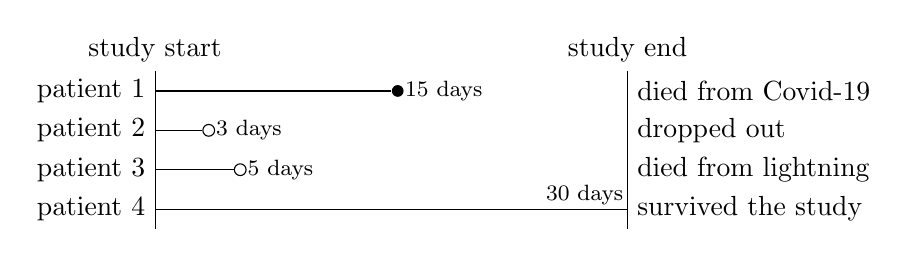
\begin{tikzpicture}
        \node[above] (start) at (0,-0.25) {study start};
        \node[above] (end) at (6,-0.25) {study end};
        \draw (start) -- (start |- ,-2.25);
        \draw (end) -- (end |- ,-2.25);
        \draw (start |- ,-.5) node[left] {patient 1} -- (3,-.5)   node[right,circle,inner sep=1.5pt,fill=black] {} node[right=1.5pt] {\footnotesize 15 days};
        \draw (start |- ,-1) node[left] {patient 2} -- (.6,-1)    node[right,circle,inner sep=1.5pt,draw=black] {} node[right=1.5pt] {\footnotesize 3 days};
        \draw (start |- ,-1.5) node[left] {patient 3} -- (1,-1.5) node[right,circle,inner sep=1.5pt,draw=black] {} node[right=1.5pt] {\footnotesize 5 days};
        \draw (start |- ,-2) node[left] {patient 4} -- (6,-2)                                                      node[above left=-2pt and -2pt]  {\footnotesize 30 days};
        \node[right] at (end |- ,-.5) {died from Covid-19};
        \node[right] at (end |- ,-1) {dropped out};
        \node[right] at (end |- ,-1.5) {died from lightning};
        \node[right] at (end |- ,-2) {survived the study};
    \end{tikzpicture}
    \pause
    The \textbf{time} is the number of days since testing positive for Covid-19.

    The \textbf{event} is whether the patient died due to Covid-19.
    \pause

    \begin{exampleblock}{Time-to-event data}
        \centering
        \begin{tabular}{c|c|c}
            patient & time & event \\
            \hline
            1 & 15 & yes \\
            2 & \only<3>{?}\only<4>{$[0,3]$} & \only<3>{?}\only<4>{no} \\
            3 & \only<3>{?}\only<4>{$[0,5)$} & \only<3>{?}\only<4>{no} \\
            4 & \only<3>{?}\only<4>{$[0,30]$} & no \\
        \end{tabular}
    \end{exampleblock}
\end{frame}

\begin{frame}{Censoring}
    We just saw examples of \textbf{right-censored} data.
    
    TODO
\end{frame}

\section{Survival function}
\begin{frame}{Survival function}
    Let $T$ be a continuous random variable representing survival time.

    The \textbf{survival function} $S(t)$ is the probability that an individual will survive past time $t$. 
    % i.e. survive until at least $t$.
    \pause
    \begin{block}{Survival function}
        $$S(t) = \prob{T > t}$$
    \end{block}
\end{frame}

\begin{frame}{Survival curve}
    \centering
    \begin{tikzpicture}
        \begin{axis}[xmin=0, ymin=0,xlabel=$t$ (time),ylabel=survival]
            \addplot [no markers, const plot, red] table [x=time,y=survival,col sep=comma] {surv_data1.csv};
            \legend{$S(t)$}
            \addplot [only marks, mark=+] table [x=time,y expr={(\thisrow{event}==0 ? \thisrow{survival} : inf )},col sep=comma] {surv_data1.csv};
        \end{axis}
    \end{tikzpicture}
\end{frame}

\begin{frame}{Modelling the survival function}
    The \textbf{Kaplan-Meier estimator} provides a non-parametric estimate of the survival function $S(t)$ using the survival curve.
    \pause
    \begin{block}{Kaplan-Meier estimator}
        \begin{align*}
            \hat{S}(t) = \prod_{i:t_i \leq t} \left( 1 - \frac{d_i}{n_i} \right)
        \end{align*}
        where
        \begin{itemize}
            \item $t_i$ is an event time
            \item $d_i$ is the number of deaths at time $t_i$
            \item $n_i$ is the number of individuals \emph{known to have survived} until $t_i$
        \end{itemize}
    \end{block}
\end{frame}
\begin{frame}{Survival curve and Kaplan-Meier estimator}
    \centering
    \begin{tikzpicture}
        \begin{axis}[xmin=0, ymin=0,xlabel=$t$ (time),ylabel=survival]
            \addplot [no markers, const plot, red] table [x=time,y=survival,col sep=comma] {surv_data1.csv};
            \addplot [no markers, const plot, blue] table [x=time,y=km,col sep=comma] {surv_data1.csv};
            \legend{$S(t)$,$\hat{S}(t)$}
            \addplot [only marks, mark=+] table [x=time,y expr={(\thisrow{event}==0 ? \thisrow{survival} : inf )},col sep=comma] {surv_data1.csv};
            \addplot [only marks, mark=+] table [x=time,y expr={(\thisrow{event}==0 ? \thisrow{km} : inf )},col sep=comma] {surv_data1.csv};
        \end{axis}
    \end{tikzpicture}
\end{frame}
\note[itemize]{
    \item When there is no censoring, $S(t)=\hat{S}(t)$.
    \item Commonly used to compare two study populations.
    \item Does not control for covariates.
}

\section{Hazard function}
\begin{frame}{Hazard function}
    The \textbf{hazard function} expresses the
    \emph{\highlight<7>{instantaneous rate} of occurence} of the event.
    \pause

    \highlight<5>{Supposing an individual survived until time $t$},
    it expresses the \highlight<4>{probability of dying within a short additional time $dt$},
    \highlight<6>{per unit time}.
    \pause
    \begin{block}{Hazard function}
        \begin{align*}
            \lambda(t)
            &= \hidelight<7>{\lim_{dt\to 0}}
                \frac{\prob{\hidelight<4>{t \leq T \leq t+dt} | \hidelight<5>{\highlight<8>{T \geq t}}}}{\hidelight<6>{dt}}\\
            \uncover<8->{
            &= \lim_{dt\to 0}
                \frac{\prob{t \leq T \leq t+dt}}{dt \cdot \only<8>{\highlight{\prob{T \geq t}}}\only<9->{\highlight<9>{S(t)}}}
            }
        \end{align*}
    \end{block}
\end{frame}

\begin{frame}{Cox proportional hazards model}
    
\end{frame}

% \section{Comparing survival distributions}
% Logrank

\end{document}